Auto-WEKA contains a GUI to allow for easy execution of experiments. To launch the GUI, you need to execute the class \classname{autoweka.ui.Launcher}. This can be done by running the command \cmdline{java -jar autoweka.jar}, or using one of the Auto-WEKA scripts. This brings up the following window that allows you to configure your experiment, run your experiment, and finally get the best set of hyperparameters that were found. Auto-WEKA features a wizard mode that uses presets to help get experiments running as quick as possible. Additionally, the launcher also provides a shortcut to launching the standard WEKA UI.

\begin{center}
  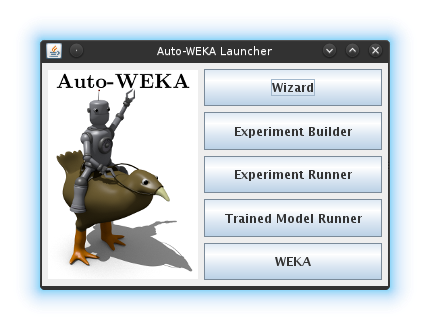
\includegraphics[scale=0.75]{guiscreens/launcher.png}
\end{center}


\subsection{Wizard}

The wizard allows for easy execution of experiments, targeted towards use cases where minimal input is required from the user. After pointing the wizard at the training data (in WEKA's ARFF data format), the user just has to pick the preset that best suits their resource limits. (Note that for larger datasets,  you will not achieve good results by using very small time limits). Pressing the ``Run Experiment'' button will cause Auto-WEKA to use the optimisation method SMAC (See Section~\ref{sec:smbo}) to find hyperparemter settings with good accuracy (for classification) or RMSE (for regression). Once the optimisation has completed, the wizard will indicate what method and hyperparameters were selected, and allow for predictions on new datasets using the trained method.

\begin{center}
  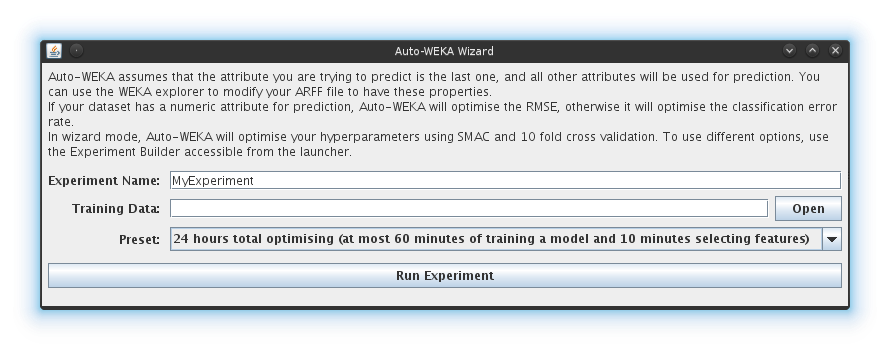
\includegraphics[scale=0.7]{guiscreens/wizard.png}
\end{center}

\subsection{Experiment Builder}

The Experiment Builder has three pages. On the first page, you specify the the location of the training data in the ARFF format. Auto-WEKA GUI assumes that the attribute you are attempting to predict is last attribute in the file,  you may need to use the WEKA UI to reorder your dataset. Additionally, you can specify the test data to use (this is only ever used in the analysis stage). If you do not specify any test data, Auto-WEKA just uses the training data instead. You can also set up the way that the optimisation method will use the training data,  through the use of an ``instance generator''. After picking the desired method, you can fine tune the method's settings by clicking on the ``Edit'' button. A more detailed explanation of each instance generator and its associated options can be found in Section~\ref{sec:instancegenerators}. Once you have made your choices, press the ``Next'' button.

\begin{center}
  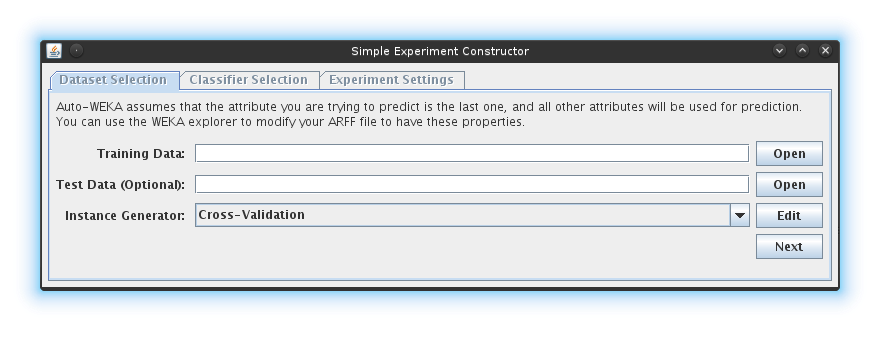
\includegraphics[scale=0.7]{guiscreens/builder-dataset.png}
\end{center}

Next Auto-WEKA allows you to limit the choice of classifiers that it will consider during for the SMBO method. The second page allows you to select which methods you would like, by control/shift clicking on the different class names to limit your selection. We recommend that you should keep all the methods selected unless you have a very specific reason for not using a particular method. Detailed about which classifiers are not applicable are printed to the system console. Once you have made your selections,  press the ``Next'' button.

\begin{center}
  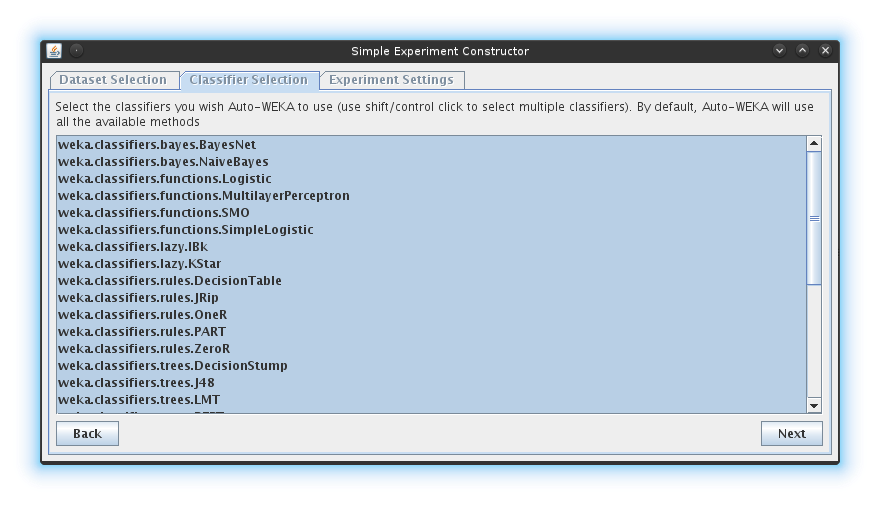
\includegraphics[scale=0.7]{guiscreens/builder-classifier.png}
\end{center}

The last page allows you to specify your experiment settings. The ``output folder'' is the folder where the sub-folder containing all of the experiment data will be produced. Change the ``Result Metric'' to one that is applicable to your dataset. After you select your optimisation method, you can fine tune specific settings by clicking on the edit button. These settings are detailed for each  method in Section~\ref{sec:smbo}. The Optimisation timeout is the number of hours that you are willing to give the optimiser to perform the hyperparameter search. The training memory limit and training run timeout are the resource constraints that are placed on the individual run of a classification or regression method that the optimisation method will perform (and it should be allowed to perform many of them). The attribute selection check box indicates to Auto-WEKA if the hyperparameter search should also be performed over WEKA's methods for transforming/selecting attributes in the dataset. The attribute selection timeout is only used when attribute selection is enabled, and is the maximum number of minutes that will be used to perform the attribute selection for each run of a hyperparameter configuration.

\begin{center}
  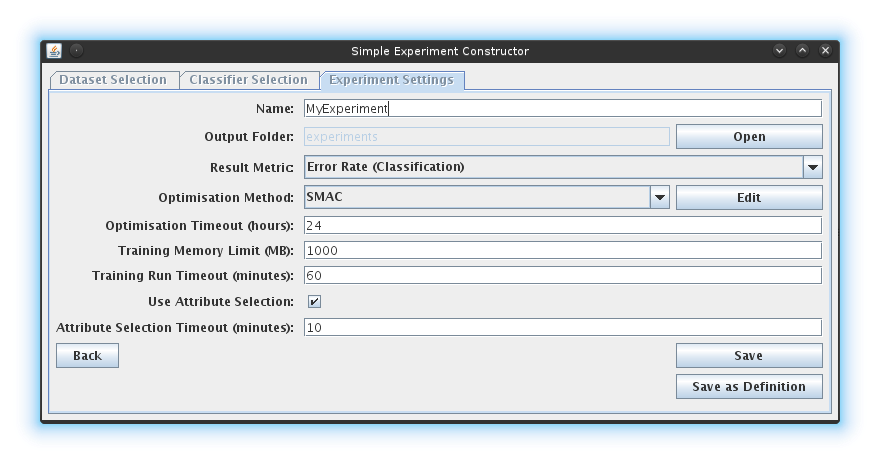
\includegraphics[scale=0.7]{guiscreens/builder-experiment.png}
\end{center}

Finally, you can either choose to fully instantiate the experiment by clicking on the ``Save'' button (which converts all paths to absolute paths) and sets up the folders for the experiment,  or you can choose to create a portable experiment definition by clicking the ``Save as Definition'' button. The experiment definition file can then be moved to a different environment,  or be modified to facilitate batch experiments. See Section~\ref{sec:experimentdefs} for more details.

\subsection{Experiment Runner}

The experiment runner provides an easy way to run a fully instantiated Auto-WEKA experiment. Simply select the folder containing the \file{.experiment} file, enter in a integer for a seed, and push the run button. For example, if your directory structure looks as follows:
\begin{verbatim}
  experiments/
     MyExperiment/
        MyExperiment.experiment
        ....
\end{verbatim}
The folder \file{experiments/MyExperiment} should be selected in the open file dialog.

\begin{center}
  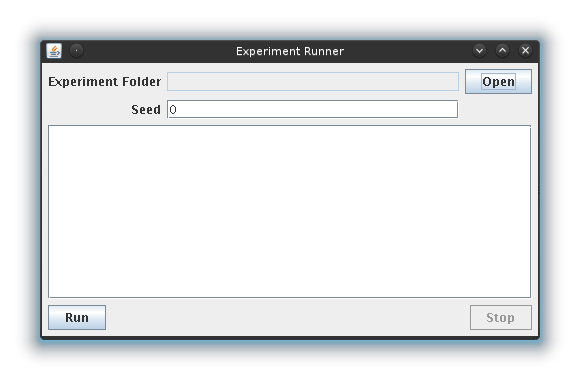
\includegraphics[scale=0.7]{guiscreens/runner.png}
\end{center}

After pressing the run button, the log screen will begin filling up with the output of the optimisation method. Consult the documentation that came with the optimisation method for an explanation of what appears.

Once the time budget has been exhausted, Auto-WEKA will begin training a model using all the training data and the best hyperparameters. If a testing set was provided, Auto-WEKA will print out some basic statistics on the performance of the trained model on the data.

\begin{aside}
  Sometimes the Stop button doesn't succeed in terminating the running process - if this is the case, you'll have to use the various tools of your OS to ensure that the optimisation process is terminated.
\end{aside}

\subsection{Trained Model Runner}

Since Auto-WEKA exploits parallelism by running the optimisation method with different seeds, after running your experiment a few times with unique seeds, you'll want to use the best hyperparameters found to make predictions on new data. After opening up the folder containing the \file{.experiment}, Auto-WEKA selects the hyperparameters that have the best error estimate. The hyperparameters are then displayed, so you can use them in WEKA's explorer (if you right click on any of the text boxes that contain arguments,  WEKA allows you to insert the command line string into it).

\begin{center}
  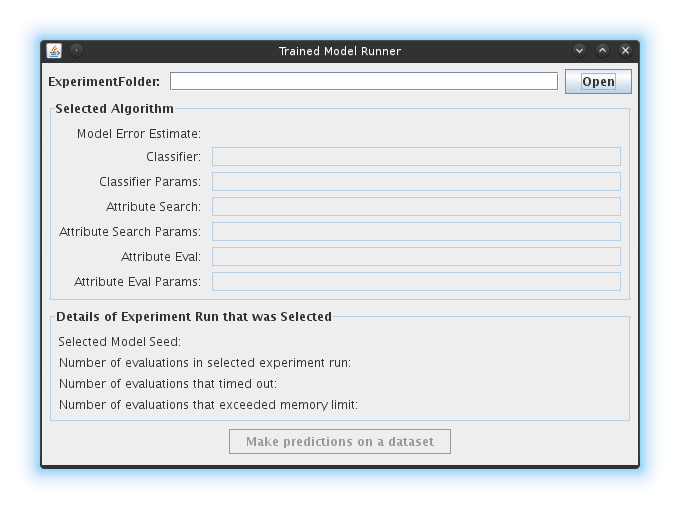
\includegraphics[scale=0.65]{guiscreens/modelrunner.png}
\end{center}

Additionally, you can provide new datasets (in ARFF format),  and use the trained model to make predictions (the results are saved as a CSV). If attribute selection was used,  this will be applied to the dataset before it is passed off to the model. Note that the format of the testing set needs to match the format of the training data exactly, otherwise you will likely get very strange predictions/cryptic error messages. 